\subsection{Secondary-Output Load and Thermal Tests}
\label{sec:res-v2-secondary-load}

The electronic load was connected to the V2 secondary output. At
approximately \SI{240}{\volt} AC and \SI{50}{\hertz}, increasing the load
current from \SI{1.86}{\ampere} to \SI{10.01}{\ampere} raised the calculated
secondary power from \SI{48.68}{\watt} to \SI{137.08}{\watt}. The secondary
voltage fell from \SI{26.14}{\volt} to \SI{13.69}{\volt} over this sequence
(\cref{tab:v2-secondary-load,fig:v2-secondary-load-performance}). At
\SI{20.07}{\volt}, the load drew \SI{4.29}{\ampere}, giving
\SI{86.17}{\watt}. The higher-power points were therefore reached with
increasing voltage droop.

\begin{table}[htbp]
\centering
\small
\setlength{\tabcolsep}{4pt}
\caption{AC input, secondary-load readings, and thermal-region maxima during the V2 load sequence. Input voltage was approximately \SI{240}{\volt} at \SI{50}{\hertz}.}
\label{tab:v2-secondary-load}
\begin{tabular}{@{}rrrrrrrr@{}}
\toprule
Capture & $P_{\mathrm{in}}$ & $V_{\mathrm{sec}}$ & $I_{\mathrm{sec}}$ & $P_{\mathrm{sec}}$ & $\eta$ & Bridge R3 & Secondary R1\\
 & (W) & (V) & (A) & (W) & (\%) & ($^\circ$C) & ($^\circ$C)\\
\midrule
015 & 64.352 & 26.14 & 1.86 & 48.68 & 75.7 & 65.1 & 50.3\\
017 & 95.142\textsuperscript{*} & 21.36 & 3.31 & 70.75 & 74.4\textsuperscript{*} & 83.9 & 57.2\\
018 & 106.731 & 20.07 & 4.29 & 86.17 & 80.7 & 68.2 & 59.7\\
019 & 121.899 & 18.46 & 5.27 & 97.35 & 79.9 & 73.2 & 69.4\\
020 & 140.565 & 16.87 & 6.51 & 109.87 & 78.2 & 74.5 & 81.6\\
021 & 168.859 & 14.92 & 8.51 & 127.05 & 75.2 & 75.6 & 88.7\\
022 & 189.180 & 13.69 & 10.01 & 137.08 & 72.5 & 73.7 & 98.3\\
\bottomrule
\end{tabular}
\par\vspace{0.4em}
\begin{minipage}{\linewidth}\footnotesize
$P_{\mathrm{sec}}$ is calculated from the electronic-load voltage and current; $\eta=100P_{\mathrm{sec}}/P_{\mathrm{in}}$ is an estimate.
\textsuperscript{*}Capture 017 reports \SI{95.142}{\watt} input, while its \SI{239.99}{\volt} and \SI{0.39}{\ampere} readings give \SI{93.60}{\volt\ampere}. The input reading and associated efficiency need checking.
\end{minipage}
\end{table}


In the thermal images in \cref{fig:v2-secondary-load-thermal}, the input-bridge
region R3 reached \SI{83.9}{\celsius} near
\SI{70.75}{\watt}. Its maxima at the subsequent higher-power points were
lower, between \SI{68.2}{\celsius} and \SI{75.6}{\celsius}. The secondary
region R1 became progressively hotter, rising from \SI{50.3}{\celsius} to
\SI{98.3}{\celsius}.

None of the load points reached thermal equilibrium. The sequence includes
both load changes and continued heating, so the temperatures cannot be
treated as settled values for each power level. Diode selection and the
current and thermal paths around the rectifiers require further work.
The tests show that the leakage-only stage can transfer more than
\SI{100}{\watt} to a secondary load, although voltage droop and continued
heating remain.

\begin{figure}[htbp]
\centering
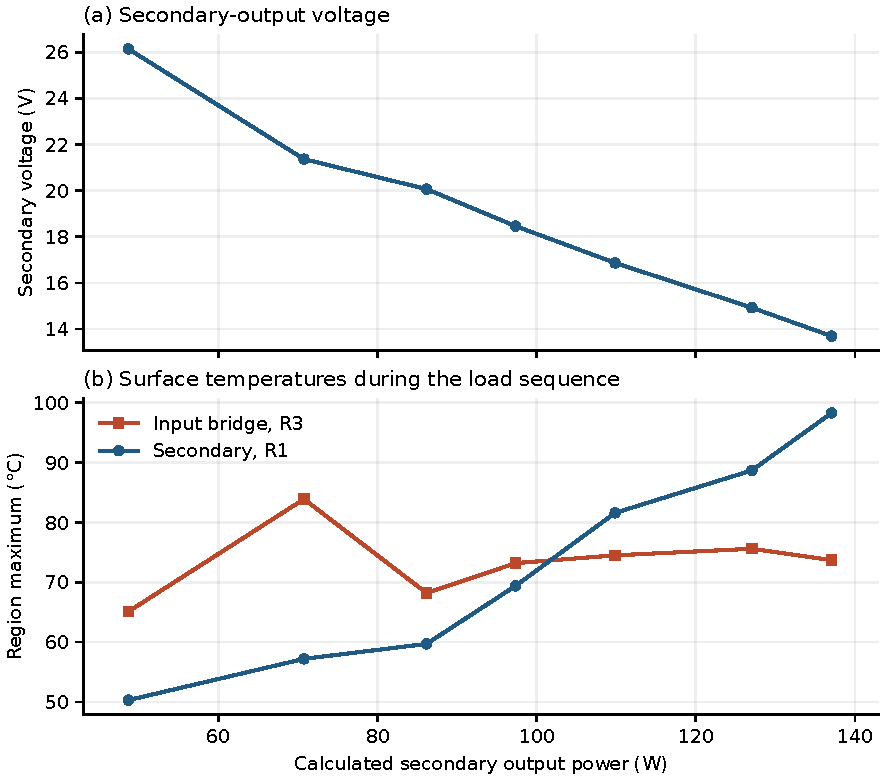
\includegraphics[width=\linewidth]{Data/measurements/v2_load_thermal/load_performance.pdf}
\caption{Secondary voltage and thermal-region maxima during the increasing-load sequence. Lines connect successive readings. R3 covers the input bridge and R1 the secondary area.}
\label{fig:v2-secondary-load-performance}
\end{figure}
\FloatBarrier

\begin{figure}[p]
\centering
\begin{subfigure}{0.78\linewidth}
\centering
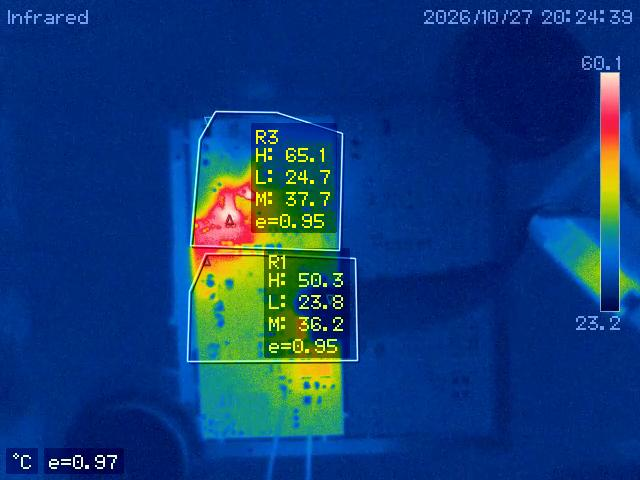
\includegraphics[width=\linewidth]{Data/measurements/v2_load_thermal/thermal/Capture 015-thermal.jpg}
\caption{Capture 015: \SI{48.68}{\watt} at the secondary load.}
\end{subfigure}
\par\vspace{0.8em}
\begin{subfigure}{0.78\linewidth}
\centering
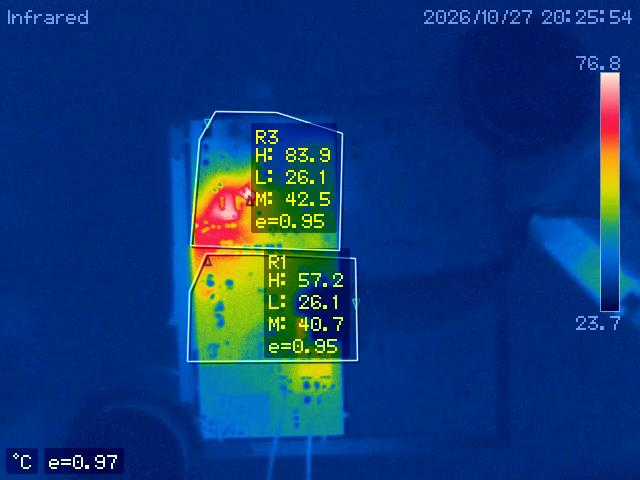
\includegraphics[width=\linewidth]{Data/measurements/v2_load_thermal/thermal/Capture 017-thermal.jpg}
\caption{Capture 017: \SI{70.75}{\watt} at the secondary load.}
\end{subfigure}
\par\vspace{0.8em}
\caption{V2 thermal images during secondary-output loading. R3 covers the input bridge and R1 the secondary area.}
\label{fig:v2-secondary-load-thermal}
\end{figure}
\begin{figure}[p]
\centering
\ContinuedFloat
\begin{subfigure}{0.78\linewidth}
\centering
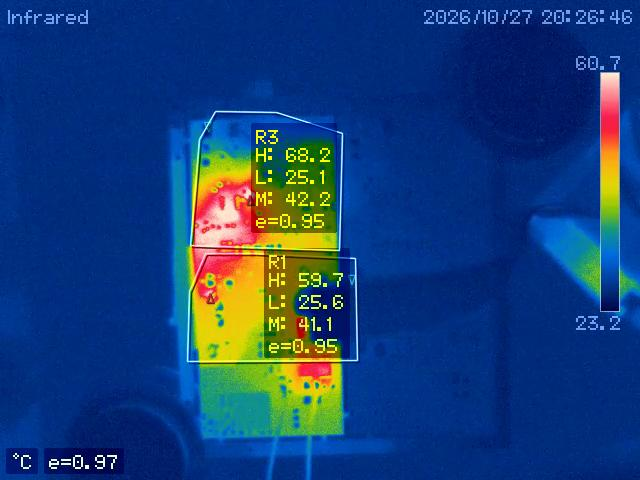
\includegraphics[width=\linewidth]{Data/measurements/v2_load_thermal/thermal/Capture 018-thermal.jpg}
\caption{Capture 018: \SI{86.17}{\watt} at the secondary load.}
\end{subfigure}
\par\vspace{0.8em}
\begin{subfigure}{0.78\linewidth}
\centering
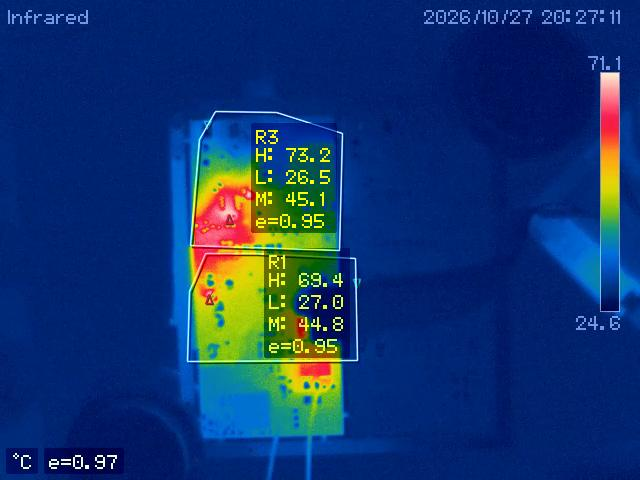
\includegraphics[width=\linewidth]{Data/measurements/v2_load_thermal/thermal/Capture 019-thermal.jpg}
\caption{Capture 019: \SI{97.35}{\watt} at the secondary load.}
\end{subfigure}
\par\vspace{0.8em}
\caption{V2 thermal images during secondary-output loading (continued). R3 covers the input bridge and R1 the secondary area.}
\end{figure}
\begin{figure}[p]
\centering
\ContinuedFloat
\begin{subfigure}{0.78\linewidth}
\centering
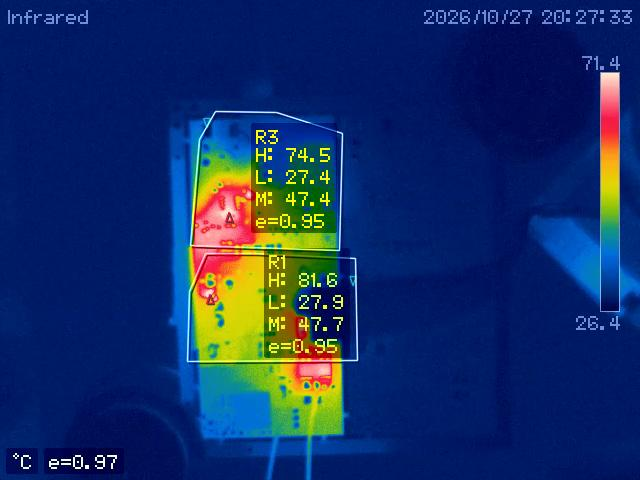
\includegraphics[width=\linewidth]{Data/measurements/v2_load_thermal/thermal/Capture 020-thermal.jpg}
\caption{Capture 020: \SI{109.87}{\watt} at the secondary load.}
\end{subfigure}
\par\vspace{0.8em}
\begin{subfigure}{0.78\linewidth}
\centering
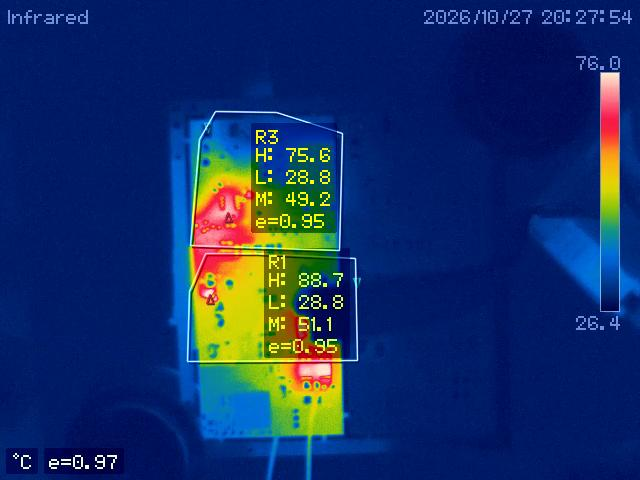
\includegraphics[width=\linewidth]{Data/measurements/v2_load_thermal/thermal/Capture 021-thermal.jpg}
\caption{Capture 021: \SI{127.05}{\watt} at the secondary load.}
\end{subfigure}
\par\vspace{0.8em}
\caption{V2 thermal images during secondary-output loading (continued). R3 covers the input bridge and R1 the secondary area.}
\end{figure}
\begin{figure}[p]
\centering
\ContinuedFloat
\begin{subfigure}{0.78\linewidth}
\centering
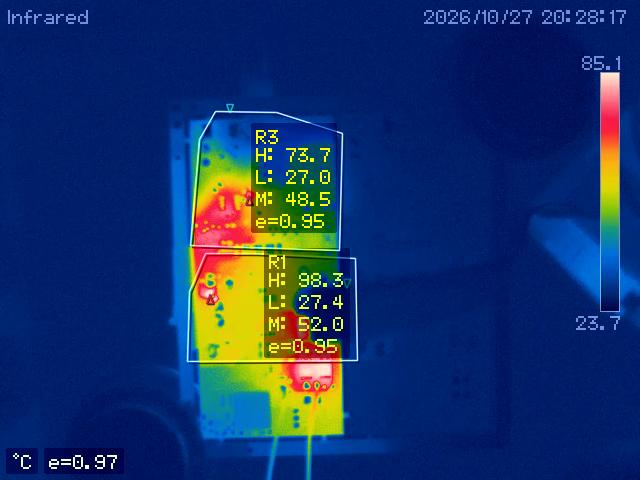
\includegraphics[width=\linewidth]{Data/measurements/v2_load_thermal/thermal/Capture 022-thermal.jpg}
\caption{Capture 022: \SI{137.08}{\watt} at the secondary load.}
\end{subfigure}
\par\vspace{0.8em}
\caption{V2 thermal images during secondary-output loading (continued). R3 covers the input bridge and R1 the secondary area.}
\end{figure}
\FloatBarrier

